\chapter{Molecular Dynamics Simulations}
% Motivate MD simulations
\begin{outline}
\1 Molecular dynamics simulations are a useful tool to study the structure, dynamics, and interaction of biomolecules. MD simulations employ an empirical mathematical function to describe the atomic interactions in a molecular system, and together with classical laws of Newtonian mechanics, atomic trajectories of motion are generated. Thermodynamic and kinetic properties can then be extracted as time averages from these trajectories and used to make a number of predictions that are often experimentally challenging to observe or measure.

\1 MD simulation studies have been useful in studying many existing fundamental problems of biology and biochemistry, including protein dynamics and function, protein folding, biomolecular self-aggregation, and protein-ligand binding.
% Study protein dynamics - importance of protein dynamics.
\end{outline}

\section{Methodological Details} % (fold)
% Describe the details of molecular dynamics simulations

% A set of numerical computation algorithm which solves numerically solves the N-body problem. Solves a system of Newton's equations of motion, and provides the time-trajectory of atoms with femtosecond time resolution. 

% The integration algorithm is XXX. Time steps used are typically 2 femtoseconds to capture the hydrogen bond vibrational motion. [MORE DETAILS AND EQUATIONS HERE] [Ref: Chris Madill's and Tom's thesis]
% Details of the mathematics (need to review the basic theory + Taylor series expansion) - get a book - tomorrow maybe?

% The assumption at a hand-wave level adapted from Tom's thesis
\begin{outline}
	\1 Why is MD correct? Describe the fundamental assumptions of MD. Here, I want to give the readers who aren't familiar with the methodological details of MD a sense of the rigorousness of MD.
	
	\1 The Born-Oppenheimer approximation: electronic and nuclear motions are uncoupled, and therefore can be treated separately. 

	\1 MD does not account for the movement of electrons. Although electrons are not taken into account in MD simulations, their presence is implicitly accounted for via the use of potential energy functions.  Atomic nuclei can be treated as classical particles.

% \2 Review the basic derivations of MD simulation equations and why they work:
%   \3 Assume a small integration step (why is 2 fs chosen it is both biological and for numerical stability purposes). Roughly MD follows these steps:
%     \4 F = -grad E, where E is given by the force field potential energy function.
%     \4 Determine acceleration for each atom from the forces on each atom
%     \4 From acceleration determine momentum 
%     \4 Determine positions

% - Relationship between force and energy 
% - Relationship between momentum and velocity 
% - Why numerical approach must be used (no analytical solution for N > 2)
% - How is the force field plugged into the general algorithm.

  \1 Application of an empirical force field can be used approximate atomic interactions in the system. A force field typically has many parameters which need to be calculated. One approach to do this is to fit to quantum mechanical calculations.  Often, force fields are iteratively improved by predicting experimentally observable quantities for small compounds, and adjusting the fit based on comparisons of these computationally predicted quantities with experimental measurements.
  
  \1 There many different force fields (AMBER, Gromos etc), each differing slightly in the potential energy function and its parameterization. In this thesis we performed all of our simulations using the force field OPLS-AA/L.

  \1 Force field potential energy function
  % \[ V(R) = bonds + angles + impropers + dihedrals + pair interactions \]
  \begin{equation}
    \begin{split}
          E = \sum_{bonds} k_b(b-b_0)^2 
          + \sum_{angles} k_{\theta}(\theta - \theta_{0})^2 \\
          + \sum_{dihedrals} k_{\chi}(1 + cos(n\chi - \delta)) 
          + \sum_{impropers} k_{\gamma}(\phi - \phi_{0})^2 \\
          + \sum_{nonbonded} \frac{q_1q_2}{er} \\
          + \sum_{nonbonded} \epsilon [(\frac{r_{min}}{r})^{12} - 2(\frac{r_{min}}{r})^6]
    \end{split}
  \end{equation}
\end{outline}

% How to run a MD simulation 
% \1 Steps to produce a molecular simulation:
%   \2 First take a structure from crystallography or NMR, or homology-modelling data.
%   \2 In the algorithm, the forces acting on each atom are estimated from [insert equation here]

\section{Challenges and limitations of MD simulations}

\begin{outline}
	\1 MD is computationally challenging because of limitations in length and time scales.
	
		\2 Length scale. Large systems are too complex to obtain statistics and quantitative predictions.
			
		% Evaluating the convergence of simulations is still a challenge
		\2 Time scale. Relevant biochemical reactions such as protein folding happens on the time scale of milliseconds, hours, and days. Currently with MD simulations, we are routinely able to approach the microsecond time scale, massive computing power is still insufficient to observe phenomena on the millisecond timescale. % Ref: DE Shaw Research.
		\2 Obtaining convergence. Explain why this is difficult, in particular for systems with disordered peptides.
	\1 Limitations in the accuracy of current force fields.
\end{outline}		

\section{Application of MD: structure-based drug discovery}
\begin{outline}
% \1 (Why computational?) Can help us get protein dynamics is important for understanding protein function. We want to understand protein function because we want to be able to design drugs to cure diseases.

% \1 A important application of MD simulation in biochemistry is the predicting of protein-ligand binding free energies.
	\1 A broad application of simulations of proteins is to computationally design drugs and combining that with structure-based drug design. In recent years structure-based computer modeling of protein-ligand interactions have become a core component of modern drug discovery. 

	\1 Current drug discovery platform. Typically, the first step in drug discovery is to identifying a target, a putative binding site.  Then, solve the X-ray crystal structure of the target.
  % [See Tom's thesis]
	
	\1 Ligands which may act as potential drugs typically have high binding affinity to the binding site. The goal is to find high specificity inhibitor of a protein (usually an enzyme). The binding free energy is an important quantity which can be used to evaluate how well a ligand binds. One method of estimating binding affinity is by using computational docking methods, where the binding affinity is typically estimated without taking into account of protein dynamics.  Although docking is computationally less expensive, it is inaccurate for identifying true drug candidates because binding often involves crucial changes in protein conformation.

	\1 With computer hardware becoming faster and cheaper, MD simulation and modeling can be used to rapidly prototype experimental ideas -- for example, one can perform computational alchemy, that is, ``mutate'' residues to test various hypotheses. Furthermore, simulations may be used to determine whether a chemical change will produce a more potent drug candidate.
	
	\1 Currently state of the art computational binding studies take into the account of change in protein conformation. MD simulations is an effective method, where the protein and drug is allowed to relax and freely move about in the system.

	\1 However, in the case of understanding a specific binding reaction (eg. when developing an enzyme inhibitor), the ability to observe the relevant binding events is a low probability event on the timescale achievable in our simulations. Therefore, it is  impractical in this case to solely apply brute-force sampling techniques to determine binding free energies.

	  \2 Methods used to determine binding free energies using simulations:
	  % \3 Linear interaction energy -- Out of scope
	  % \3 MM/PBSA - no explicit account for solvents -- Out of scope
	  	\3 Thermodynamic perturbation \cite{Gilson:2007hz}
			\4 thermodynamic integration
			\4 free energy perturbation
\end{outline}

\section{Review of MD studies of amyloid inhibition by small molecules}
% MD studies using brute-force sampling. Aid in medicinal chemistry by making suggestions for how to design new AD drugs.

\begin{outline}
	%  Excerpt from Transfer proposal
	\1 In recent years, molecular dynamics simulations have been intensively used to investigate the molecular basis of the structure and stability of amyloid fibrils. 
	
	\1 MD simulations of Congo red binding have been done with the protofibril-like crystal structure composed of the segment GNNQQNY.\{Wu, 2007 \#621\}
	
	\1 A recent simulation study of an N-methylated peptide with A$\beta$16-22 models of amyloid aggregates has provided insight into the possible mechanism of action of peptide inhibitors of amyloid formation.\{Soto, 2007 \#597\} This peptide inhibitor was shown to preferentially bind monomers to form dimers, possibly acting to inhibit fibril formation by sequestering monomers. However, peptide-based inhibitors have poor pharmacological profiles as they are actively broken down by proteases in the stomach and are difficult to transport across the blood-brain barrier. In addition, these peptide inhibitors specifically target A$\beta$ and thus do not have the potential to treat multiple amyloid diseases.
\end{outline}


\section{Thesis objectives and rationale}
% Understanding amyloid inhibition in the context of the framework of traditional enzyme inhibition mechanism
\subsection{Challenges of amyloid inhibition}
\begin{outline}
       % However, most of these studies were focused on A$\beta$ and large A$\beta$ aggregates,\{Fawzi, 2008 \#553;Esposito, 2008 \#567;Sgourakis, 2007 \#609;Wei, 2006 \#656;Tarus, 2006 \#628 Karsai, 2006 \#658\} and thus, were computationally limited by the complexity of the molecular systems.


    \1 The protein-ligand binding model developed to understand enzyme inhibition cannot be directly applied to understand the molecular mechanism of amyloid inhibition by small molecules. 
    
      \2 Amyloid inhibitors are found to be very weak binders. How do non-specific inhibitors act as a drug? And how do we approach this with MD simulations?
      
      \2  Because the A$\beta$ amyloid aggregate pathway encompasses a variety of species, some of which has no folded structure, a single conformation cannot be assumed for binding. Furthermore, structural information of amyloidogenic species lags behind those of enzymes, which tends to be globular proteins amenable for X-ray crystallography. This means that the putative binding sites are not known.
      
      \2 The structural disorder of the peptides involved poses a challenge for obtaining converged properties from MD simulations. 
    
    	\1 A$\beta$ peptides are completely disordered.  We also do not know what the binding site looks like, where it is located on these structures.
    	
    \1 To date, few studies have attempted to provide statistically meaningful results pertaining to general mechanisms of protein self-aggregation and amyloid formation. Furthermore, despite the abundance of MD studies of A$\beta$, few studies have systematically examined the mechanism of action of small molecule inhibitors of amyloids

    \1 In AD, there is the added challenge of the drug being able to cross the brain barrier, while remaining non-neurotoxic.  What kind of drugs cross the BBB?  Typically hydrophobic drugs.
\end{outline}    

\subsection{Study Design and Rationale}
\begin{outline}
	\1 Here describe in detail how I designed my study to circumvent the challenges presented by the amyloid inhibition problem, and the limitations  of MD simulations. At this point, clearly explain and discuss my study design and rationale. (Fig.~\ref{fig:rationale})

  \begin{figure}
    \centering
    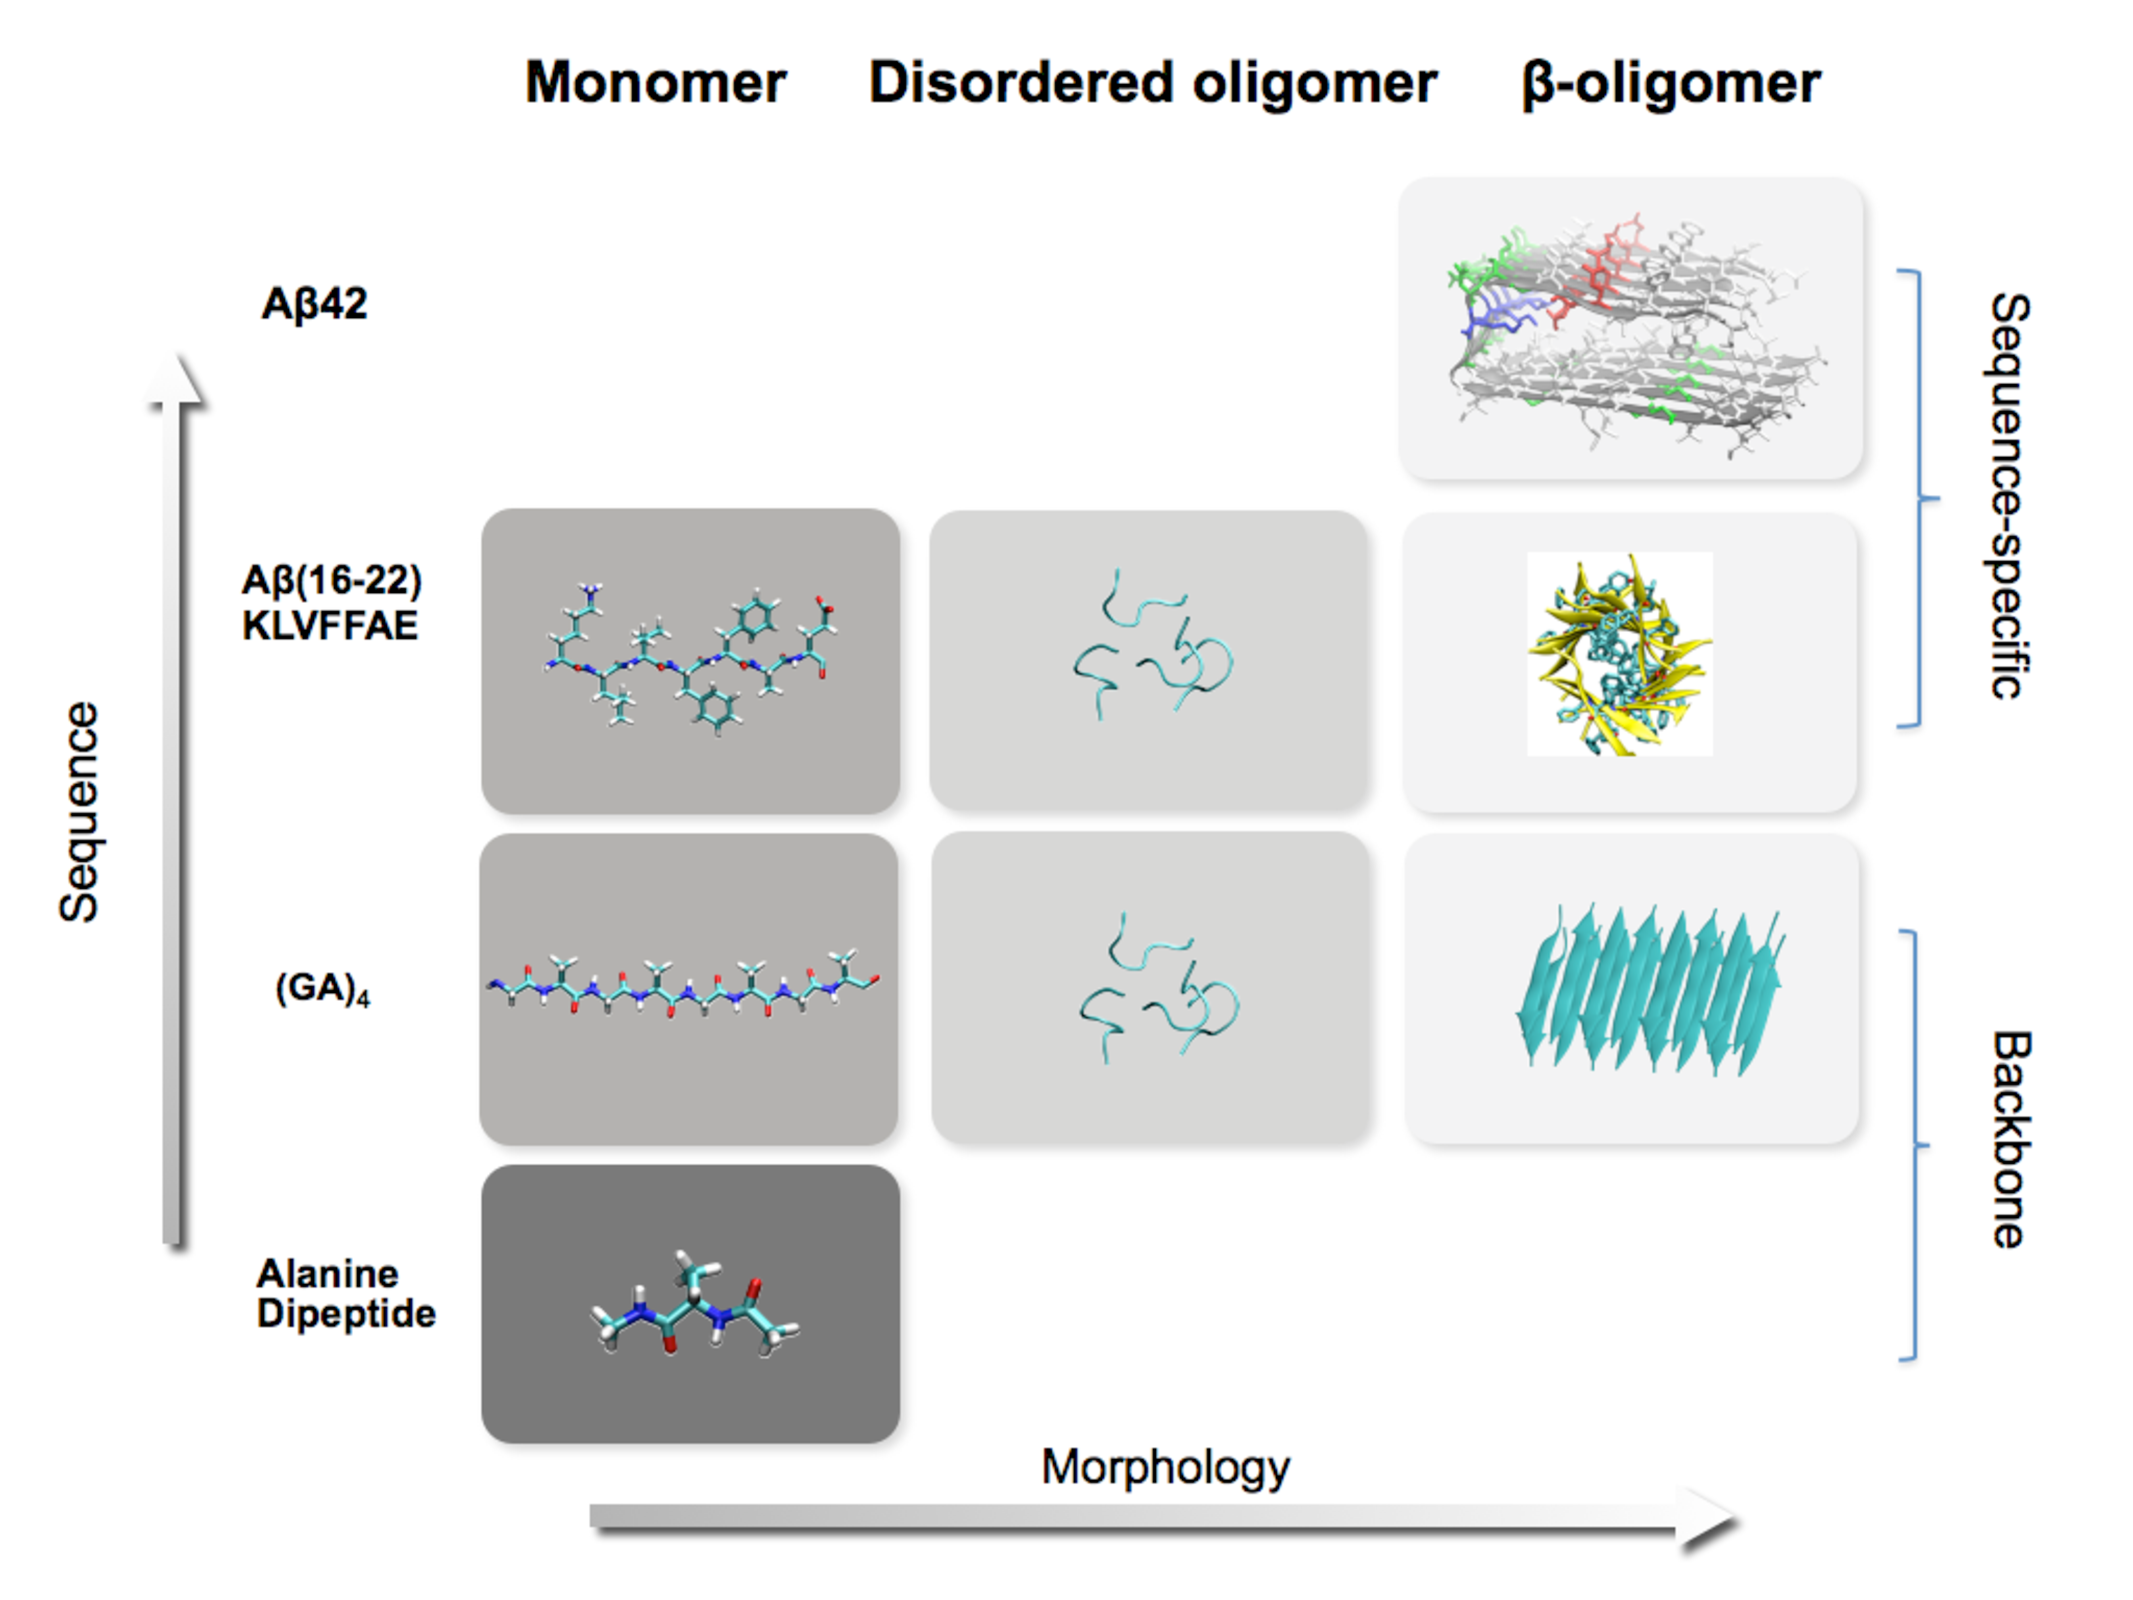
\includegraphics[width=6in]{figures/introduction/matrix.pdf}
    \caption[Rationale]{Shows the progression from small, model systems to larger and structurally more complex systems involving the full-length A$\beta$42 peptide.}
    \label{fig:rationale}
  \end{figure}

	\1 Beginning with the simplest model systems for an amyloidogenic peptide, the alanine dipeptide, we systematically examine binding of inositol with systems of both increasing sequence and structural complexity.

	% Use brute force simulations
	\1 We exploit conventional MD simulation techniques because simulation approaches used for understanding enzyme-ligand binding is not applicable. 
	
	\1 Instead, we use conventional MD simulations and repeats of independent simulations to determine the binding modes, and binding equilibria of inositol with amyloidogenic peptides and aggregates of A$\beta$.
\end{outline}

\addcontentsline{toc}{section}{Bibliography}
\bibliographystyle{plain}
\bibliography{chapter1}